\documentclass[1p]{elsarticle_modified}
%\bibliographystyle{elsarticle-num}

%\usepackage[colorlinks]{hyperref}
%\usepackage{abbrmath_seonhwa} %\Abb, \Ascr, \Acal ,\Abf, \Afrak
\usepackage{amsfonts}
\usepackage{amssymb}
\usepackage{amsmath}
\usepackage{amsthm}
\usepackage{scalefnt}
\usepackage{amsbsy}
\usepackage{kotex}
\usepackage{caption}
\usepackage{subfig}
\usepackage{color}
\usepackage{graphicx}
\usepackage{xcolor} %% white, black, red, green, blue, cyan, magenta, yellow
\usepackage{float}
\usepackage{setspace}
\usepackage{hyperref}

\usepackage{tikz}
\usetikzlibrary{arrows}

\usepackage{multirow}
\usepackage{array} % fixed length table
\usepackage{hhline}

%%%%%%%%%%%%%%%%%%%%%
\makeatletter
\renewcommand*\env@matrix[1][\arraystretch]{%
	\edef\arraystretch{#1}%
	\hskip -\arraycolsep
	\let\@ifnextchar\new@ifnextchar
	\array{*\c@MaxMatrixCols c}}
\makeatother %https://tex.stackexchange.com/questions/14071/how-can-i-increase-the-line-spacing-in-a-matrix
%%%%%%%%%%%%%%%

\usepackage[normalem]{ulem}

\newcommand{\msout}[1]{\ifmmode\text{\sout{\ensuremath{#1}}}\else\sout{#1}\fi}
%SOURCE: \msout is \stkout macro in https://tex.stackexchange.com/questions/20609/strikeout-in-math-mode

\newcommand{\cancel}[1]{
	\ifmmode
	{\color{red}\msout{#1}}
	\else
	{\color{red}\sout{#1}}
	\fi
}

\newcommand{\add}[1]{
	{\color{blue}\uwave{#1}}
}

\newcommand{\replace}[2]{
	\ifmmode
	{\color{red}\msout{#1}}{\color{blue}\uwave{#2}}
	\else
	{\color{red}\sout{#1}}{\color{blue}\uwave{#2}}
	\fi
}

\newcommand{\Sol}{\mathcal{S}} %segment
\newcommand{\D}{D} %diagram
\newcommand{\A}{\mathcal{A}} %arc


%%%%%%%%%%%%%%%%%%%%%%%%%%%%%5 test

\def\sl{\operatorname{\textup{SL}}(2,\Cbb)}
\def\psl{\operatorname{\textup{PSL}}(2,\Cbb)}
\def\quan{\mkern 1mu \triangleright \mkern 1mu}

\theoremstyle{definition}
\newtheorem{thm}{Theorem}[section]
\newtheorem{prop}[thm]{Proposition}
\newtheorem{lem}[thm]{Lemma}
\newtheorem{ques}[thm]{Question}
\newtheorem{cor}[thm]{Corollary}
\newtheorem{defn}[thm]{Definition}
\newtheorem{exam}[thm]{Example}
\newtheorem{rmk}[thm]{Remark}
\newtheorem{alg}[thm]{Algorithm}

\newcommand{\I}{\sqrt{-1}}
\begin{document}

%\begin{frontmatter}
%
%\title{Boundary parabolic representations of knots up to 8 crossings}
%
%%% Group authors per affiliation:
%\author{Yunhi Cho} 
%\address{Department of Mathematics, University of Seoul, Seoul, Korea}
%\ead{yhcho@uos.ac.kr}
%
%
%\author{Seonhwa Kim} %\fnref{s_kim}}
%\address{Center for Geometry and Physics, Institute for Basic Science, Pohang, 37673, Korea}
%\ead{ryeona17@ibs.re.kr}
%
%\author{Hyuk Kim}
%\address{Department of Mathematical Sciences, Seoul National University, Seoul 08826, Korea}
%\ead{hyukkim@snu.ac.kr}
%
%\author{Seokbeom Yoon}
%\address{Department of Mathematical Sciences, Seoul National University, Seoul, 08826,  Korea}
%\ead{sbyoon15@snu.ac.kr}
%
%\begin{abstract}
%We find all boundary parabolic representation of knots up to 8 crossings.
%
%\end{abstract}
%\begin{keyword}
%    \MSC[2010] 57M25 
%\end{keyword}
%
%\end{frontmatter}

%\linenumbers
%\tableofcontents
%
\newcommand\colored[1]{\textcolor{white}{\rule[-0.35ex]{0.8em}{1.4ex}}\kern-0.8em\color{red} #1}%
%\newcommand\colored[1]{\textcolor{white}{ #1}\kern-2.17ex	\textcolor{white}{ #1}\kern-1.81ex	\textcolor{white}{ #1}\kern-2.15ex\color{red}#1	}

{\Large $\underline{12a_{0256}~(K12a_{0256})}$}

\setlength{\tabcolsep}{10pt}
\renewcommand{\arraystretch}{1.6}
\vspace{1cm}\begin{tabular}{m{100pt}>{\centering\arraybackslash}m{274pt}}
\multirow{5}{120pt}{
	\centering
	\includegraphics[width=112pt]{../../../GIT/diagram.site/Diagrams/png/1057_12a_0256.png}\\
\ \ \ A knot diagram\footnotemark}&
\allowdisplaybreaks
\textbf{Linearized knot diagam} \\
\cline{2-2}
 &
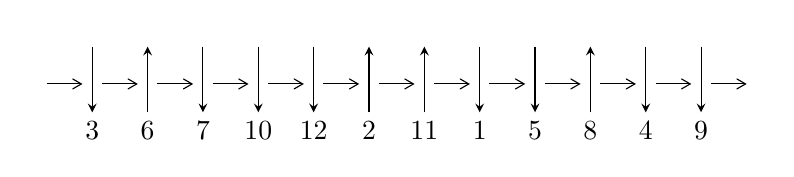
\begin{tikzpicture}[x=20pt, y=17pt]
	% nodes
	\node (C0) at (0, 0) {};
	\node (C1) at (1, 0) {};
	\node (C1U) at (1, +1) {};
	\node (C1D) at (1, -1) {3};

	\node (C2) at (2, 0) {};
	\node (C2U) at (2, +1) {};
	\node (C2D) at (2, -1) {6};

	\node (C3) at (3, 0) {};
	\node (C3U) at (3, +1) {};
	\node (C3D) at (3, -1) {7};

	\node (C4) at (4, 0) {};
	\node (C4U) at (4, +1) {};
	\node (C4D) at (4, -1) {10};

	\node (C5) at (5, 0) {};
	\node (C5U) at (5, +1) {};
	\node (C5D) at (5, -1) {12};

	\node (C6) at (6, 0) {};
	\node (C6U) at (6, +1) {};
	\node (C6D) at (6, -1) {2};

	\node (C7) at (7, 0) {};
	\node (C7U) at (7, +1) {};
	\node (C7D) at (7, -1) {11};

	\node (C8) at (8, 0) {};
	\node (C8U) at (8, +1) {};
	\node (C8D) at (8, -1) {1};

	\node (C9) at (9, 0) {};
	\node (C9U) at (9, +1) {};
	\node (C9D) at (9, -1) {5};

	\node (C10) at (10, 0) {};
	\node (C10U) at (10, +1) {};
	\node (C10D) at (10, -1) {8};

	\node (C11) at (11, 0) {};
	\node (C11U) at (11, +1) {};
	\node (C11D) at (11, -1) {4};

	\node (C12) at (12, 0) {};
	\node (C12U) at (12, +1) {};
	\node (C12D) at (12, -1) {9};
	\node (C13) at (13, 0) {};

	% arrows
	\draw[->,>={angle 60}]
	(C0) edge (C1) (C1) edge (C2) (C2) edge (C3) (C3) edge (C4) (C4) edge (C5) (C5) edge (C6) (C6) edge (C7) (C7) edge (C8) (C8) edge (C9) (C9) edge (C10) (C10) edge (C11) (C11) edge (C12) (C12) edge (C13) ;	\draw[->,>=stealth]
	(C1U) edge (C1D) (C2D) edge (C2U) (C3U) edge (C3D) (C4U) edge (C4D) (C5U) edge (C5D) (C6D) edge (C6U) (C7D) edge (C7U) (C8U) edge (C8D) (C9U) edge (C9D) (C10D) edge (C10U) (C11U) edge (C11D) (C12U) edge (C12D) ;
	\end{tikzpicture} \\
\hhline{~~} \\& 
\textbf{Solving Sequence} \\ \cline{2-2} 
 &
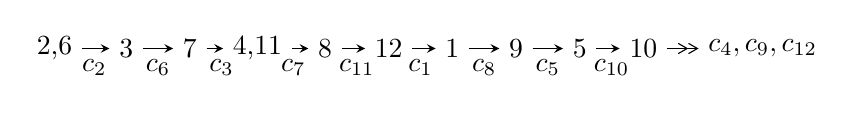
\begin{tikzpicture}[x=23pt, y=7pt]
	% node
	\node (A0) at (-1/8, 0) {2,6};
	\node (A1) at (1, 0) {3};
	\node (A2) at (2, 0) {7};
	\node (A3) at (49/16, 0) {4,11};
	\node (A4) at (33/8, 0) {8};
	\node (A5) at (41/8, 0) {12};
	\node (A6) at (49/8, 0) {1};
	\node (A7) at (57/8, 0) {9};
	\node (A8) at (65/8, 0) {5};
	\node (A9) at (73/8, 0) {10};
	\node (C1) at (1/2, -1) {$c_{2}$};
	\node (C2) at (3/2, -1) {$c_{6}$};
	\node (C3) at (5/2, -1) {$c_{3}$};
	\node (C4) at (29/8, -1) {$c_{7}$};
	\node (C5) at (37/8, -1) {$c_{11}$};
	\node (C6) at (45/8, -1) {$c_{1}$};
	\node (C7) at (53/8, -1) {$c_{8}$};
	\node (C8) at (61/8, -1) {$c_{5}$};
	\node (C9) at (69/8, -1) {$c_{10}$};
	\node (A10) at (11, 0) {$c_{4},c_{9},c_{12}$};

	% edge
	\draw[->,>=stealth]	
	(A0) edge (A1) (A1) edge (A2) (A2) edge (A3) (A3) edge (A4) (A4) edge (A5) (A5) edge (A6) (A6) edge (A7) (A7) edge (A8) (A8) edge (A9) ;
	\draw[->>,>={angle 60}]	
	(A9) edge (A10);
\end{tikzpicture} \\ 

\end{tabular} \\

\footnotetext{
The image of knot diagram is generated by the software ``\textbf{Draw programme}" developed by Andrew Bartholomew(\url{http://www.layer8.co.uk/maths/draw/index.htm\#Running-draw}), where we modified some parts for our purpose(\url{https://github.com/CATsTAILs/LinksPainter}).
}\phantom \\ \newline 
\centering \textbf{Ideals for irreducible components\footnotemark of $X_{\text{par}}$} 
 
\begin{align*}
I^u_{1}&=\langle 
2.56758\times10^{188} u^{136}+1.42936\times10^{189} u^{135}+\cdots+2.47840\times10^{187} b-1.95610\times10^{188},\\
\phantom{I^u_{1}}&\phantom{= \langle  }2.04389\times10^{188} u^{136}+1.15337\times10^{189} u^{135}+\cdots+2.47840\times10^{187} a-8.69370\times10^{187},\;u^{137}+5 u^{136}+\cdots-3 u-1\rangle \\
I^u_{2}&=\langle 
-5 u^{26}- u^{25}+\cdots+b-6,\;-5 u^{27}-3 u^{26}+\cdots+a-4,\;u^{28}+8 u^{26}+\cdots-2 u+1\rangle \\
\\
\end{align*}
\raggedright * 2 irreducible components of $\dim_{\mathbb{C}}=0$, with total 165 representations.\\
\footnotetext{All coefficients of polynomials are rational numbers. But the coefficients are sometimes approximated in decimal forms when there is not enough margin.}
\newpage
\renewcommand{\arraystretch}{1}
\centering \section*{I. $I^u_{1}= \langle 2.57\times10^{188} u^{136}+1.43\times10^{189} u^{135}+\cdots+2.48\times10^{187} b-1.96\times10^{188},\;2.04\times10^{188} u^{136}+1.15\times10^{189} u^{135}+\cdots+2.48\times10^{187} a-8.69\times10^{187},\;u^{137}+5 u^{136}+\cdots-3 u-1 \rangle$}
\flushleft \textbf{(i) Arc colorings}\\
\begin{tabular}{m{7pt} m{180pt} m{7pt} m{180pt} }
\flushright $a_{2}=$&$\begin{pmatrix}1\\0\end{pmatrix}$ \\
\flushright $a_{6}=$&$\begin{pmatrix}0\\u\end{pmatrix}$ \\
\flushright $a_{3}=$&$\begin{pmatrix}1\\- u^2\end{pmatrix}$ \\
\flushright $a_{7}=$&$\begin{pmatrix}u\\u\end{pmatrix}$ \\
\flushright $a_{4}=$&$\begin{pmatrix}u^4+u^2+1\\u^4\end{pmatrix}$ \\
\flushright $a_{11}=$&$\begin{pmatrix}-8.24683 u^{136}-46.5369 u^{135}+\cdots+34.6876 u+3.50779\\-10.3598 u^{136}-57.6726 u^{135}+\cdots+28.1421 u+7.89259\end{pmatrix}$ \\
\flushright $a_{8}=$&$\begin{pmatrix}1.62844 u^{136}+10.3502 u^{135}+\cdots-2.08567 u+3.05147\\-2.24765 u^{136}-7.89848 u^{135}+\cdots-14.2337 u-4.99920\end{pmatrix}$ \\
\flushright $a_{12}=$&$\begin{pmatrix}-4.73113 u^{136}-29.1031 u^{135}+\cdots+31.2965 u+2.98213\\-4.43686 u^{136}-28.1267 u^{135}+\cdots+16.0148 u+4.77163\end{pmatrix}$ \\
\flushright $a_{1}=$&$\begin{pmatrix}u^2+1\\- u^4\end{pmatrix}$ \\
\flushright $a_{9}=$&$\begin{pmatrix}-0.0634631 u^{136}-0.511369 u^{135}+\cdots+12.2936 u+6.46153\\-7.98027 u^{136}-38.7088 u^{135}+\cdots+0.862867 u-0.263602\end{pmatrix}$ \\
\flushright $a_{5}=$&$\begin{pmatrix}5.35808 u^{136}+27.7315 u^{135}+\cdots-11.7973 u+0.359303\\6.75832 u^{136}+37.5761 u^{135}+\cdots-38.0131 u-10.3110\end{pmatrix}$ \\
\flushright $a_{10}=$&$\begin{pmatrix}-0.550892 u^{136}+1.58672 u^{135}+\cdots-29.6268 u-8.41074\\3.01851 u^{136}+18.3843 u^{135}+\cdots-8.86141 u-5.99470\end{pmatrix}$\\&\end{tabular}
\flushleft \textbf{(ii) Obstruction class $= -1$}\\~\\
\flushleft \textbf{(iii) Cusp Shapes $= 3.41230 u^{136}+7.78483 u^{135}+\cdots-25.4529 u-5.81017$}\\~\\
\newpage\renewcommand{\arraystretch}{1}
\flushleft \textbf{(iv) u-Polynomials at the component}\newline \\
\begin{tabular}{m{50pt}|m{274pt}}
Crossings & \hspace{64pt}u-Polynomials at each crossing \\
\hline $$\begin{aligned}c_{1}\end{aligned}$$&$\begin{aligned}
&u^{137}+71 u^{136}+\cdots-11 u-1
\end{aligned}$\\
\hline $$\begin{aligned}c_{2},c_{6}\end{aligned}$$&$\begin{aligned}
&u^{137}-5 u^{136}+\cdots-3 u+1
\end{aligned}$\\
\hline $$\begin{aligned}c_{3}\end{aligned}$$&$\begin{aligned}
&u^{137}+5 u^{136}+\cdots-28109 u+49282
\end{aligned}$\\
\hline $$\begin{aligned}c_{4},c_{9}\end{aligned}$$&$\begin{aligned}
&u^{137}- u^{136}+\cdots+37207 u+14092
\end{aligned}$\\
\hline $$\begin{aligned}c_{5}\end{aligned}$$&$\begin{aligned}
&u^{137}+18 u^{135}+\cdots+38195407 u+7601057
\end{aligned}$\\
\hline $$\begin{aligned}c_{7},c_{10}\end{aligned}$$&$\begin{aligned}
&u^{137}+6 u^{136}+\cdots-20079 u+3169
\end{aligned}$\\
\hline $$\begin{aligned}c_{8},c_{12}\end{aligned}$$&$\begin{aligned}
&u^{137}+3 u^{136}+\cdots-1611854 u+205619
\end{aligned}$\\
\hline $$\begin{aligned}c_{11}\end{aligned}$$&$\begin{aligned}
&u^{137}+5 u^{136}+\cdots+361656 u+26671
\end{aligned}$\\
\hline
\end{tabular}\\~\\
\newpage\renewcommand{\arraystretch}{1}
\flushleft \textbf{(v) Riley Polynomials at the component}\newline \\
\begin{tabular}{m{50pt}|m{274pt}}
Crossings & \hspace{64pt}Riley Polynomials at each crossing \\
\hline $$\begin{aligned}c_{1}\end{aligned}$$&$\begin{aligned}
&y^{137}- y^{136}+\cdots+61 y-1
\end{aligned}$\\
\hline $$\begin{aligned}c_{2},c_{6}\end{aligned}$$&$\begin{aligned}
&y^{137}+71 y^{136}+\cdots-11 y-1
\end{aligned}$\\
\hline $$\begin{aligned}c_{3}\end{aligned}$$&$\begin{aligned}
&y^{137}-73 y^{136}+\cdots+30864949201 y-2428715524
\end{aligned}$\\
\hline $$\begin{aligned}c_{4},c_{9}\end{aligned}$$&$\begin{aligned}
&y^{137}+103 y^{136}+\cdots-3967076151 y-198584464
\end{aligned}$\\
\hline $$\begin{aligned}c_{5}\end{aligned}$$&$\begin{aligned}
&y^{137}+36 y^{136}+\cdots-2839868740482897 y-57776067517249
\end{aligned}$\\
\hline $$\begin{aligned}c_{7},c_{10}\end{aligned}$$&$\begin{aligned}
&y^{137}+90 y^{136}+\cdots-824301543 y-10042561
\end{aligned}$\\
\hline $$\begin{aligned}c_{8},c_{12}\end{aligned}$$&$\begin{aligned}
&y^{137}+93 y^{136}+\cdots-669185450976 y-42279173161
\end{aligned}$\\
\hline $$\begin{aligned}c_{11}\end{aligned}$$&$\begin{aligned}
&y^{137}-17 y^{136}+\cdots+62854050382 y-711342241
\end{aligned}$\\
\hline
\end{tabular}\\~\\
\newpage\flushleft \textbf{(vi) Complex Volumes and Cusp Shapes}
$$\begin{array}{c|c|c}  
\text{Solutions to }I^u_{1}& \I (\text{vol} + \sqrt{-1}CS) & \text{Cusp shape}\\
 \hline 
\begin{aligned}
u &= -0.533319 + 0.849244 I \\
a &= \phantom{-}0.116988 - 0.644715 I \\
b &= \phantom{-}0.815465 - 1.064700 I\end{aligned}
 & -1.12416 - 2.04890 I & \phantom{-0.000000 } 0 \\ \hline\begin{aligned}
u &= -0.533319 - 0.849244 I \\
a &= \phantom{-}0.116988 + 0.644715 I \\
b &= \phantom{-}0.815465 + 1.064700 I\end{aligned}
 & -1.12416 + 2.04890 I & \phantom{-0.000000 } 0 \\ \hline\begin{aligned}
u &= \phantom{-}0.502796 + 0.853410 I \\
a &= \phantom{-}0.984550 + 0.293887 I \\
b &= \phantom{-}0.182920 - 0.493163 I\end{aligned}
 & \phantom{-}0.28337 - 1.41442 I & \phantom{-0.000000 } 0 \\ \hline\begin{aligned}
u &= \phantom{-}0.502796 - 0.853410 I \\
a &= \phantom{-}0.984550 - 0.293887 I \\
b &= \phantom{-}0.182920 + 0.493163 I\end{aligned}
 & \phantom{-}0.28337 + 1.41442 I & \phantom{-0.000000 } 0 \\ \hline\begin{aligned}
u &= -0.957173 + 0.102971 I \\
a &= -0.25823 - 1.86243 I \\
b &= -0.162071 - 0.899505 I\end{aligned}
 & \phantom{-}3.30511 - 0.01751 I & \phantom{-0.000000 } 0 \\ \hline\begin{aligned}
u &= -0.957173 - 0.102971 I \\
a &= -0.25823 + 1.86243 I \\
b &= -0.162071 + 0.899505 I\end{aligned}
 & \phantom{-}3.30511 + 0.01751 I & \phantom{-0.000000 } 0 \\ \hline\begin{aligned}
u &= -0.304693 + 0.910206 I \\
a &= -0.26481 - 1.50058 I \\
b &= \phantom{-}0.668726 - 0.857128 I\end{aligned}
 & \phantom{-}2.61366 - 5.14297 I & \phantom{-0.000000 } 0 \\ \hline\begin{aligned}
u &= -0.304693 - 0.910206 I \\
a &= -0.26481 + 1.50058 I \\
b &= \phantom{-}0.668726 + 0.857128 I\end{aligned}
 & \phantom{-}2.61366 + 5.14297 I & \phantom{-0.000000 } 0 \\ \hline\begin{aligned}
u &= \phantom{-}0.596239 + 0.863165 I \\
a &= -0.958277 + 0.025577 I \\
b &= -1.86008 + 0.32518 I\end{aligned}
 & \phantom{-}7.73934 - 0.81536 I & \phantom{-0.000000 } 0 \\ \hline\begin{aligned}
u &= \phantom{-}0.596239 - 0.863165 I \\
a &= -0.958277 - 0.025577 I \\
b &= -1.86008 - 0.32518 I\end{aligned}
 & \phantom{-}7.73934 + 0.81536 I & \phantom{-0.000000 } 0\\
 \hline 
 \end{array}$$\newpage$$\begin{array}{c|c|c}  
\text{Solutions to }I^u_{1}& \I (\text{vol} + \sqrt{-1}CS) & \text{Cusp shape}\\
 \hline 
\begin{aligned}
u &= \phantom{-}0.069847 + 1.050040 I \\
a &= \phantom{-}0.0056226 + 0.0646777 I \\
b &= -1.068510 + 0.267075 I\end{aligned}
 & -0.0265712 - 0.0562753 I & \phantom{-0.000000 } 0 \\ \hline\begin{aligned}
u &= \phantom{-}0.069847 - 1.050040 I \\
a &= \phantom{-}0.0056226 - 0.0646777 I \\
b &= -1.068510 - 0.267075 I\end{aligned}
 & -0.0265712 + 0.0562753 I & \phantom{-0.000000 } 0 \\ \hline\begin{aligned}
u &= -0.325030 + 0.878832 I \\
a &= \phantom{-}0.456202 - 0.441515 I \\
b &= \phantom{-}0.286899 - 0.477025 I\end{aligned}
 & -0.54203 - 1.42582 I & \phantom{-0.000000 } 0 \\ \hline\begin{aligned}
u &= -0.325030 - 0.878832 I \\
a &= \phantom{-}0.456202 + 0.441515 I \\
b &= \phantom{-}0.286899 + 0.477025 I\end{aligned}
 & -0.54203 + 1.42582 I & \phantom{-0.000000 } 0 \\ \hline\begin{aligned}
u &= \phantom{-}0.617489 + 0.700364 I \\
a &= \phantom{-}0.17956 - 1.41511 I \\
b &= -0.130881 - 0.287691 I\end{aligned}
 & \phantom{-}8.20953 + 5.56566 I & \phantom{-0.000000 } 0 \\ \hline\begin{aligned}
u &= \phantom{-}0.617489 - 0.700364 I \\
a &= \phantom{-}0.17956 + 1.41511 I \\
b &= -0.130881 + 0.287691 I\end{aligned}
 & \phantom{-}8.20953 - 5.56566 I & \phantom{-0.000000 } 0 \\ \hline\begin{aligned}
u &= \phantom{-}0.887754 + 0.262797 I \\
a &= \phantom{-}0.12921 + 2.14576 I \\
b &= \phantom{-}0.179272 + 0.677955 I\end{aligned}
 & -1.93538 - 7.48838 I & \phantom{-0.000000 } 0 \\ \hline\begin{aligned}
u &= \phantom{-}0.887754 - 0.262797 I \\
a &= \phantom{-}0.12921 - 2.14576 I \\
b &= \phantom{-}0.179272 - 0.677955 I\end{aligned}
 & -1.93538 + 7.48838 I & \phantom{-0.000000 } 0 \\ \hline\begin{aligned}
u &= \phantom{-}0.756689 + 0.764410 I \\
a &= -0.110558 - 0.663621 I \\
b &= \phantom{-}0.216956 + 0.337434 I\end{aligned}
 & \phantom{-}6.38454 - 5.71250 I & \phantom{-0.000000 } 0 \\ \hline\begin{aligned}
u &= \phantom{-}0.756689 - 0.764410 I \\
a &= -0.110558 + 0.663621 I \\
b &= \phantom{-}0.216956 - 0.337434 I\end{aligned}
 & \phantom{-}6.38454 + 5.71250 I & \phantom{-0.000000 } 0\\
 \hline 
 \end{array}$$\newpage$$\begin{array}{c|c|c}  
\text{Solutions to }I^u_{1}& \I (\text{vol} + \sqrt{-1}CS) & \text{Cusp shape}\\
 \hline 
\begin{aligned}
u &= -0.988134 + 0.432807 I \\
a &= -0.160589 + 1.032590 I \\
b &= \phantom{-}0.242816 + 0.384392 I\end{aligned}
 & \phantom{-}3.73770 - 1.79692 I & \phantom{-0.000000 } 0 \\ \hline\begin{aligned}
u &= -0.988134 - 0.432807 I \\
a &= -0.160589 - 1.032590 I \\
b &= \phantom{-}0.242816 - 0.384392 I\end{aligned}
 & \phantom{-}3.73770 + 1.79692 I & \phantom{-0.000000 } 0 \\ \hline\begin{aligned}
u &= \phantom{-}0.575110 + 0.713441 I \\
a &= -0.217900 + 0.741038 I \\
b &= \phantom{-}0.99074 + 1.18801 I\end{aligned}
 & \phantom{-}0.68274 + 5.78618 I & \phantom{-0.000000 } 0 \\ \hline\begin{aligned}
u &= \phantom{-}0.575110 - 0.713441 I \\
a &= -0.217900 - 0.741038 I \\
b &= \phantom{-}0.99074 - 1.18801 I\end{aligned}
 & \phantom{-}0.68274 - 5.78618 I & \phantom{-0.000000 } 0 \\ \hline\begin{aligned}
u &= -0.869875 + 0.251926 I \\
a &= \phantom{-}0.08200 - 2.32233 I \\
b &= \phantom{-}0.361982 - 0.715554 I\end{aligned}
 & \phantom{-}2.71900 + 13.79220 I & \phantom{-0.000000 } 0 \\ \hline\begin{aligned}
u &= -0.869875 - 0.251926 I \\
a &= \phantom{-}0.08200 + 2.32233 I \\
b &= \phantom{-}0.361982 + 0.715554 I\end{aligned}
 & \phantom{-}2.71900 - 13.79220 I & \phantom{-0.000000 } 0 \\ \hline\begin{aligned}
u &= \phantom{-}0.490407 + 0.755910 I \\
a &= \phantom{-}0.636976 + 1.124530 I \\
b &= \phantom{-}1.099390 + 0.433924 I\end{aligned}
 & \phantom{-}3.99446 + 2.04024 I & \phantom{-0.000000 } 0 \\ \hline\begin{aligned}
u &= \phantom{-}0.490407 - 0.755910 I \\
a &= \phantom{-}0.636976 - 1.124530 I \\
b &= \phantom{-}1.099390 - 0.433924 I\end{aligned}
 & \phantom{-}3.99446 - 2.04024 I & \phantom{-0.000000 } 0 \\ \hline\begin{aligned}
u &= \phantom{-}0.718798 + 0.835116 I \\
a &= -0.150342 - 0.075852 I \\
b &= -1.263490 - 0.320415 I\end{aligned}
 & \phantom{-}6.16457 + 11.21360 I & \phantom{-0.000000 } 0 \\ \hline\begin{aligned}
u &= \phantom{-}0.718798 - 0.835116 I \\
a &= -0.150342 + 0.075852 I \\
b &= -1.263490 + 0.320415 I\end{aligned}
 & \phantom{-}6.16457 - 11.21360 I & \phantom{-0.000000 } 0\\
 \hline 
 \end{array}$$\newpage$$\begin{array}{c|c|c}  
\text{Solutions to }I^u_{1}& \I (\text{vol} + \sqrt{-1}CS) & \text{Cusp shape}\\
 \hline 
\begin{aligned}
u &= -0.680528 + 0.577464 I \\
a &= \phantom{-}0.432488 + 0.843523 I \\
b &= \phantom{-}0.145641 + 0.260873 I\end{aligned}
 & \phantom{-}3.38601 - 0.98367 I & \phantom{-0.000000 } 0 \\ \hline\begin{aligned}
u &= -0.680528 - 0.577464 I \\
a &= \phantom{-}0.432488 - 0.843523 I \\
b &= \phantom{-}0.145641 - 0.260873 I\end{aligned}
 & \phantom{-}3.38601 + 0.98367 I & \phantom{-0.000000 } 0 \\ \hline\begin{aligned}
u &= \phantom{-}0.354562 + 1.052920 I \\
a &= \phantom{-}0.343872 - 0.019856 I \\
b &= \phantom{-}0.104155 - 0.950397 I\end{aligned}
 & -1.331140 - 0.354042 I & \phantom{-0.000000 } 0 \\ \hline\begin{aligned}
u &= \phantom{-}0.354562 - 1.052920 I \\
a &= \phantom{-}0.343872 + 0.019856 I \\
b &= \phantom{-}0.104155 + 0.950397 I\end{aligned}
 & -1.331140 + 0.354042 I & \phantom{-0.000000 } 0 \\ \hline\begin{aligned}
u &= -0.166408 + 1.098790 I \\
a &= -1.50293 - 0.36380 I \\
b &= -2.64367 - 0.36084 I\end{aligned}
 & -4.55631 - 3.25534 I & \phantom{-0.000000 } 0 \\ \hline\begin{aligned}
u &= -0.166408 - 1.098790 I \\
a &= -1.50293 + 0.36380 I \\
b &= -2.64367 + 0.36084 I\end{aligned}
 & -4.55631 + 3.25534 I & \phantom{-0.000000 } 0 \\ \hline\begin{aligned}
u &= -0.472124 + 1.038700 I \\
a &= \phantom{-}0.407735 - 1.282440 I \\
b &= -0.063430 - 0.465076 I\end{aligned}
 & \phantom{-}3.23424 - 0.51796 I & \phantom{-0.000000 } 0 \\ \hline\begin{aligned}
u &= -0.472124 - 1.038700 I \\
a &= \phantom{-}0.407735 + 1.282440 I \\
b &= -0.063430 + 0.465076 I\end{aligned}
 & \phantom{-}3.23424 + 0.51796 I & \phantom{-0.000000 } 0 \\ \hline\begin{aligned}
u &= \phantom{-}0.712987 + 0.446274 I \\
a &= \phantom{-}1.111570 + 0.012824 I \\
b &= \phantom{-}0.352809 - 0.679136 I\end{aligned}
 & \phantom{-}4.76931 - 1.62940 I & \phantom{-0.000000 } 0 \\ \hline\begin{aligned}
u &= \phantom{-}0.712987 - 0.446274 I \\
a &= \phantom{-}1.111570 - 0.012824 I \\
b &= \phantom{-}0.352809 + 0.679136 I\end{aligned}
 & \phantom{-}4.76931 + 1.62940 I & \phantom{-0.000000 } 0\\
 \hline 
 \end{array}$$\newpage$$\begin{array}{c|c|c}  
\text{Solutions to }I^u_{1}& \I (\text{vol} + \sqrt{-1}CS) & \text{Cusp shape}\\
 \hline 
\begin{aligned}
u &= -0.667112 + 0.501243 I \\
a &= \phantom{-}0.911117 - 0.658420 I \\
b &= \phantom{-}0.759339 + 0.465298 I\end{aligned}
 & \phantom{-}5.05813 + 0.60000 I & \phantom{-0.000000 } 0 \\ \hline\begin{aligned}
u &= -0.667112 - 0.501243 I \\
a &= \phantom{-}0.911117 + 0.658420 I \\
b &= \phantom{-}0.759339 - 0.465298 I\end{aligned}
 & \phantom{-}5.05813 - 0.60000 I & \phantom{-0.000000 } 0 \\ \hline\begin{aligned}
u &= -0.546634 + 1.030390 I \\
a &= \phantom{-}0.267839 - 1.154730 I \\
b &= \phantom{-}1.10542 - 1.03275 I\end{aligned}
 & \phantom{-}3.50173 - 5.32217 I & \phantom{-0.000000 } 0 \\ \hline\begin{aligned}
u &= -0.546634 - 1.030390 I \\
a &= \phantom{-}0.267839 + 1.154730 I \\
b &= \phantom{-}1.10542 + 1.03275 I\end{aligned}
 & \phantom{-}3.50173 + 5.32217 I & \phantom{-0.000000 } 0 \\ \hline\begin{aligned}
u &= -0.378661 + 1.103420 I \\
a &= \phantom{-}0.140117 - 0.141434 I \\
b &= \phantom{-}0.023825 - 0.869305 I\end{aligned}
 & -1.35691 - 0.78518 I & \phantom{-0.000000 } 0 \\ \hline\begin{aligned}
u &= -0.378661 - 1.103420 I \\
a &= \phantom{-}0.140117 + 0.141434 I \\
b &= \phantom{-}0.023825 + 0.869305 I\end{aligned}
 & -1.35691 + 0.78518 I & \phantom{-0.000000 } 0 \\ \hline\begin{aligned}
u &= \phantom{-}0.809928 + 0.190888 I \\
a &= -0.47628 - 2.02906 I \\
b &= -0.519671 - 0.606618 I\end{aligned}
 & -4.37189 - 2.92393 I & -8.03585 + 0. I\phantom{ +0.000000I} \\ \hline\begin{aligned}
u &= \phantom{-}0.809928 - 0.190888 I \\
a &= -0.47628 + 2.02906 I \\
b &= -0.519671 + 0.606618 I\end{aligned}
 & -4.37189 + 2.92393 I & -8.03585 + 0. I\phantom{ +0.000000I} \\ \hline\begin{aligned}
u &= \phantom{-}0.419233 + 1.096630 I \\
a &= \phantom{-}3.28779 + 0.82729 I \\
b &= \phantom{-}4.00138 + 1.08547 I\end{aligned}
 & \phantom{-}1.63196 - 0.57127 I & \phantom{-0.000000 } 0 \\ \hline\begin{aligned}
u &= \phantom{-}0.419233 - 1.096630 I \\
a &= \phantom{-}3.28779 - 0.82729 I \\
b &= \phantom{-}4.00138 - 1.08547 I\end{aligned}
 & \phantom{-}1.63196 + 0.57127 I & \phantom{-0.000000 } 0\\
 \hline 
 \end{array}$$\newpage$$\begin{array}{c|c|c}  
\text{Solutions to }I^u_{1}& \I (\text{vol} + \sqrt{-1}CS) & \text{Cusp shape}\\
 \hline 
\begin{aligned}
u &= -0.309532 + 1.135070 I \\
a &= \phantom{-}0.637035 + 0.462955 I \\
b &= \phantom{-}0.92097 + 1.47589 I\end{aligned}
 & \phantom{-}2.06956 + 4.03324 I & \phantom{-0.000000 } 0 \\ \hline\begin{aligned}
u &= -0.309532 - 1.135070 I \\
a &= \phantom{-}0.637035 - 0.462955 I \\
b &= \phantom{-}0.92097 - 1.47589 I\end{aligned}
 & \phantom{-}2.06956 - 4.03324 I & \phantom{-0.000000 } 0 \\ \hline\begin{aligned}
u &= \phantom{-}0.434697 + 1.101330 I \\
a &= -1.351880 + 0.178073 I \\
b &= -2.39197 - 0.79055 I\end{aligned}
 & -3.75315 + 0.76063 I & \phantom{-0.000000 } 0 \\ \hline\begin{aligned}
u &= \phantom{-}0.434697 - 1.101330 I \\
a &= -1.351880 - 0.178073 I \\
b &= -2.39197 + 0.79055 I\end{aligned}
 & -3.75315 - 0.76063 I & \phantom{-0.000000 } 0 \\ \hline\begin{aligned}
u &= -0.766102 + 0.246672 I \\
a &= -0.63871 + 2.36043 I \\
b &= -0.737180 + 0.709707 I\end{aligned}
 & -1.48537 + 7.19229 I & -2.90359 - 6.29894 I \\ \hline\begin{aligned}
u &= -0.766102 - 0.246672 I \\
a &= -0.63871 - 2.36043 I \\
b &= -0.737180 - 0.709707 I\end{aligned}
 & -1.48537 - 7.19229 I & -2.90359 + 6.29894 I \\ \hline\begin{aligned}
u &= -0.749282 + 0.261094 I \\
a &= -1.229260 - 0.235481 I \\
b &= \phantom{-}0.372948 - 0.002355 I\end{aligned}
 & \phantom{-}6.22390 + 7.17173 I & \phantom{-}1.35640 - 5.57817 I \\ \hline\begin{aligned}
u &= -0.749282 - 0.261094 I \\
a &= -1.229260 + 0.235481 I \\
b &= \phantom{-}0.372948 + 0.002355 I\end{aligned}
 & \phantom{-}6.22390 - 7.17173 I & \phantom{-}1.35640 + 5.57817 I \\ \hline\begin{aligned}
u &= -0.450406 + 1.119820 I \\
a &= -2.04217 - 0.38943 I \\
b &= -3.24431 + 0.11454 I\end{aligned}
 & -4.22382 - 5.85372 I & \phantom{-0.000000 } 0 \\ \hline\begin{aligned}
u &= -0.450406 - 1.119820 I \\
a &= -2.04217 + 0.38943 I \\
b &= -3.24431 - 0.11454 I\end{aligned}
 & -4.22382 + 5.85372 I & \phantom{-0.000000 } 0\\
 \hline 
 \end{array}$$\newpage$$\begin{array}{c|c|c}  
\text{Solutions to }I^u_{1}& \I (\text{vol} + \sqrt{-1}CS) & \text{Cusp shape}\\
 \hline 
\begin{aligned}
u &= \phantom{-}0.474163 + 1.111140 I \\
a &= \phantom{-}1.88851 + 0.59079 I \\
b &= \phantom{-}3.19369 + 0.46268 I\end{aligned}
 & -3.45317 + 6.67791 I & \phantom{-0.000000 } 0 \\ \hline\begin{aligned}
u &= \phantom{-}0.474163 - 1.111140 I \\
a &= \phantom{-}1.88851 - 0.59079 I \\
b &= \phantom{-}3.19369 - 0.46268 I\end{aligned}
 & -3.45317 - 6.67791 I & \phantom{-0.000000 } 0 \\ \hline\begin{aligned}
u &= -0.309506 + 1.167930 I \\
a &= \phantom{-}1.60936 + 0.86298 I \\
b &= \phantom{-}2.56755 + 0.23611 I\end{aligned}
 & -5.73719 + 3.86942 I & \phantom{-0.000000 } 0 \\ \hline\begin{aligned}
u &= -0.309506 - 1.167930 I \\
a &= \phantom{-}1.60936 - 0.86298 I \\
b &= \phantom{-}2.56755 - 0.23611 I\end{aligned}
 & -5.73719 - 3.86942 I & \phantom{-0.000000 } 0 \\ \hline\begin{aligned}
u &= \phantom{-}0.483929 + 1.108490 I \\
a &= -3.12745 + 0.85374 I \\
b &= -3.96728 + 0.63687 I\end{aligned}
 & \phantom{-}2.11058 + 7.96960 I & \phantom{-0.000000 } 0 \\ \hline\begin{aligned}
u &= \phantom{-}0.483929 - 1.108490 I \\
a &= -3.12745 - 0.85374 I \\
b &= -3.96728 - 0.63687 I\end{aligned}
 & \phantom{-}2.11058 - 7.96960 I & \phantom{-0.000000 } 0 \\ \hline\begin{aligned}
u &= -0.447836 + 1.123900 I \\
a &= \phantom{-}2.17137 - 0.64014 I \\
b &= \phantom{-}3.28589 - 0.91335 I\end{aligned}
 & -4.23233 - 1.82443 I & \phantom{-0.000000 } 0 \\ \hline\begin{aligned}
u &= -0.447836 - 1.123900 I \\
a &= \phantom{-}2.17137 + 0.64014 I \\
b &= \phantom{-}3.28589 + 0.91335 I\end{aligned}
 & -4.23233 + 1.82443 I & \phantom{-0.000000 } 0 \\ \hline\begin{aligned}
u &= \phantom{-}0.579612 + 1.066840 I \\
a &= -0.372465 + 0.966588 I \\
b &= \phantom{-}0.159901 + 1.382820 I\end{aligned}
 & \phantom{-}2.94960 + 6.58219 I & \phantom{-0.000000 } 0 \\ \hline\begin{aligned}
u &= \phantom{-}0.579612 - 1.066840 I \\
a &= -0.372465 - 0.966588 I \\
b &= \phantom{-}0.159901 - 1.382820 I\end{aligned}
 & \phantom{-}2.94960 - 6.58219 I & \phantom{-0.000000 } 0\\
 \hline 
 \end{array}$$\newpage$$\begin{array}{c|c|c}  
\text{Solutions to }I^u_{1}& \I (\text{vol} + \sqrt{-1}CS) & \text{Cusp shape}\\
 \hline 
\begin{aligned}
u &= \phantom{-}0.446297 + 1.130490 I \\
a &= -0.347437 - 0.281460 I \\
b &= -0.428965 + 0.284776 I\end{aligned}
 & -4.22376 + 3.90424 I & \phantom{-0.000000 } 0 \\ \hline\begin{aligned}
u &= \phantom{-}0.446297 - 1.130490 I \\
a &= -0.347437 + 0.281460 I \\
b &= -0.428965 - 0.284776 I\end{aligned}
 & -4.22376 - 3.90424 I & \phantom{-0.000000 } 0 \\ \hline\begin{aligned}
u &= -0.628866 + 1.049280 I \\
a &= -0.509840 - 0.322071 I \\
b &= -0.802525 - 0.260188 I\end{aligned}
 & \phantom{-}2.06270 - 4.14982 I & \phantom{-0.000000 } 0 \\ \hline\begin{aligned}
u &= -0.628866 - 1.049280 I \\
a &= -0.509840 + 0.322071 I \\
b &= -0.802525 + 0.260188 I\end{aligned}
 & \phantom{-}2.06270 + 4.14982 I & \phantom{-0.000000 } 0 \\ \hline\begin{aligned}
u &= \phantom{-}0.769989 + 0.085192 I \\
a &= \phantom{-}0.69957 - 2.14608 I \\
b &= -0.334847 - 0.454878 I\end{aligned}
 & -0.21167 - 3.95519 I & -0.70872 + 4.40749 I \\ \hline\begin{aligned}
u &= \phantom{-}0.769989 - 0.085192 I \\
a &= \phantom{-}0.69957 + 2.14608 I \\
b &= -0.334847 + 0.454878 I\end{aligned}
 & -0.21167 + 3.95519 I & -0.70872 - 4.40749 I \\ \hline\begin{aligned}
u &= \phantom{-}0.690948 + 0.327915 I \\
a &= -0.534108 + 0.568309 I \\
b &= \phantom{-}0.437649 - 0.094786 I\end{aligned}
 & \phantom{-}2.37595 - 2.88460 I & -0.64698 + 3.62738 I \\ \hline\begin{aligned}
u &= \phantom{-}0.690948 - 0.327915 I \\
a &= -0.534108 - 0.568309 I \\
b &= \phantom{-}0.437649 + 0.094786 I\end{aligned}
 & \phantom{-}2.37595 + 2.88460 I & -0.64698 - 3.62738 I \\ \hline\begin{aligned}
u &= -0.761678 + 0.972727 I \\
a &= -0.513431 - 0.357447 I \\
b &= -1.164300 - 0.121244 I\end{aligned}
 & \phantom{-}2.09836 - 4.33096 I & \phantom{-0.000000 } 0 \\ \hline\begin{aligned}
u &= -0.761678 - 0.972727 I \\
a &= -0.513431 + 0.357447 I \\
b &= -1.164300 + 0.121244 I\end{aligned}
 & \phantom{-}2.09836 + 4.33096 I & \phantom{-0.000000 } 0\\
 \hline 
 \end{array}$$\newpage$$\begin{array}{c|c|c}  
\text{Solutions to }I^u_{1}& \I (\text{vol} + \sqrt{-1}CS) & \text{Cusp shape}\\
 \hline 
\begin{aligned}
u &= -0.494451 + 1.133360 I \\
a &= -0.945389 - 0.096475 I \\
b &= -1.19728 - 0.77220 I\end{aligned}
 & -0.53789 - 6.91554 I & \phantom{-0.000000 } 0 \\ \hline\begin{aligned}
u &= -0.494451 - 1.133360 I \\
a &= -0.945389 + 0.096475 I \\
b &= -1.19728 + 0.77220 I\end{aligned}
 & -0.53789 + 6.91554 I & \phantom{-0.000000 } 0 \\ \hline\begin{aligned}
u &= \phantom{-}0.535487 + 1.114710 I \\
a &= \phantom{-}0.528266 + 0.009933 I \\
b &= \phantom{-}1.046600 - 0.694471 I\end{aligned}
 & \phantom{-}0.07546 + 7.60673 I & \phantom{-0.000000 } 0 \\ \hline\begin{aligned}
u &= \phantom{-}0.535487 - 1.114710 I \\
a &= \phantom{-}0.528266 - 0.009933 I \\
b &= \phantom{-}1.046600 + 0.694471 I\end{aligned}
 & \phantom{-}0.07546 - 7.60673 I & \phantom{-0.000000 } 0 \\ \hline\begin{aligned}
u &= -0.424065 + 1.166910 I \\
a &= \phantom{-}1.82804 - 0.27571 I \\
b &= \phantom{-}2.84165 - 0.96154 I\end{aligned}
 & -4.83821 - 1.44208 I & \phantom{-0.000000 } 0 \\ \hline\begin{aligned}
u &= -0.424065 - 1.166910 I \\
a &= \phantom{-}1.82804 + 0.27571 I \\
b &= \phantom{-}2.84165 + 0.96154 I\end{aligned}
 & -4.83821 + 1.44208 I & \phantom{-0.000000 } 0 \\ \hline\begin{aligned}
u &= \phantom{-}0.025066 + 0.753968 I \\
a &= \phantom{-}0.564772 - 0.822293 I \\
b &= -0.233222 - 0.889953 I\end{aligned}
 & -0.93531 - 1.11977 I & -7.63811 + 4.58075 I \\ \hline\begin{aligned}
u &= \phantom{-}0.025066 - 0.753968 I \\
a &= \phantom{-}0.564772 + 0.822293 I \\
b &= -0.233222 + 0.889953 I\end{aligned}
 & -0.93531 + 1.11977 I & -7.63811 - 4.58075 I \\ \hline\begin{aligned}
u &= \phantom{-}0.295392 + 0.690589 I \\
a &= -0.451041 + 0.994000 I \\
b &= \phantom{-}1.086820 + 0.656532 I\end{aligned}
 & -0.14414 + 3.11446 I & -8.84863 + 1.95541 I \\ \hline\begin{aligned}
u &= \phantom{-}0.295392 - 0.690589 I \\
a &= -0.451041 - 0.994000 I \\
b &= \phantom{-}1.086820 - 0.656532 I\end{aligned}
 & -0.14414 - 3.11446 I & -8.84863 - 1.95541 I\\
 \hline 
 \end{array}$$\newpage$$\begin{array}{c|c|c}  
\text{Solutions to }I^u_{1}& \I (\text{vol} + \sqrt{-1}CS) & \text{Cusp shape}\\
 \hline 
\begin{aligned}
u &= -0.473615 + 1.159220 I \\
a &= -2.23868 - 0.05116 I \\
b &= -3.47114 - 0.04967 I\end{aligned}
 & -4.48472 - 6.82060 I & \phantom{-0.000000 } 0 \\ \hline\begin{aligned}
u &= -0.473615 - 1.159220 I \\
a &= -2.23868 + 0.05116 I \\
b &= -3.47114 + 0.04967 I\end{aligned}
 & -4.48472 + 6.82060 I & \phantom{-0.000000 } 0 \\ \hline\begin{aligned}
u &= -0.478731 + 0.568594 I \\
a &= \phantom{-}1.316230 - 0.160713 I \\
b &= \phantom{-}0.035393 + 0.245607 I\end{aligned}
 & -0.39680 - 2.11027 I & -3.71418 + 2.14261 I \\ \hline\begin{aligned}
u &= -0.478731 - 0.568594 I \\
a &= \phantom{-}1.316230 + 0.160713 I \\
b &= \phantom{-}0.035393 - 0.245607 I\end{aligned}
 & -0.39680 + 2.11027 I & -3.71418 - 2.14261 I \\ \hline\begin{aligned}
u &= \phantom{-}0.333106 + 1.214680 I \\
a &= \phantom{-}1.52890 - 0.65967 I \\
b &= \phantom{-}2.44133 - 0.21664 I\end{aligned}
 & -8.68461 + 0.83942 I & \phantom{-0.000000 } 0 \\ \hline\begin{aligned}
u &= \phantom{-}0.333106 - 1.214680 I \\
a &= \phantom{-}1.52890 + 0.65967 I \\
b &= \phantom{-}2.44133 + 0.21664 I\end{aligned}
 & -8.68461 - 0.83942 I & \phantom{-0.000000 } 0 \\ \hline\begin{aligned}
u &= \phantom{-}0.407231 + 1.196350 I \\
a &= \phantom{-}1.285220 + 0.287911 I \\
b &= \phantom{-}2.06870 + 1.29048 I\end{aligned}
 & -3.96480 + 0.12479 I & \phantom{-0.000000 } 0 \\ \hline\begin{aligned}
u &= \phantom{-}0.407231 - 1.196350 I \\
a &= \phantom{-}1.285220 - 0.287911 I \\
b &= \phantom{-}2.06870 - 1.29048 I\end{aligned}
 & -3.96480 - 0.12479 I & \phantom{-0.000000 } 0 \\ \hline\begin{aligned}
u &= -0.538558 + 1.145630 I \\
a &= \phantom{-}0.397123 + 0.477194 I \\
b &= \phantom{-}0.69365 + 1.54220 I\end{aligned}
 & \phantom{-}3.63696 - 12.02450 I & \phantom{-0.000000 } 0 \\ \hline\begin{aligned}
u &= -0.538558 - 1.145630 I \\
a &= \phantom{-}0.397123 - 0.477194 I \\
b &= \phantom{-}0.69365 - 1.54220 I\end{aligned}
 & \phantom{-}3.63696 + 12.02450 I & \phantom{-0.000000 } 0\\
 \hline 
 \end{array}$$\newpage$$\begin{array}{c|c|c}  
\text{Solutions to }I^u_{1}& \I (\text{vol} + \sqrt{-1}CS) & \text{Cusp shape}\\
 \hline 
\begin{aligned}
u &= -0.541768 + 1.153570 I \\
a &= -2.22949 + 0.90829 I \\
b &= -3.30390 + 0.95277 I\end{aligned}
 & -4.13786 - 12.09350 I & \phantom{-0.000000 } 0 \\ \hline\begin{aligned}
u &= -0.541768 - 1.153570 I \\
a &= -2.22949 - 0.90829 I \\
b &= -3.30390 - 0.95277 I\end{aligned}
 & -4.13786 + 12.09350 I & \phantom{-0.000000 } 0 \\ \hline\begin{aligned}
u &= -0.275174 + 1.252270 I \\
a &= -1.71289 - 0.25641 I \\
b &= -2.64631 + 0.39413 I\end{aligned}
 & -2.15174 + 10.09580 I & \phantom{-0.000000 } 0 \\ \hline\begin{aligned}
u &= -0.275174 - 1.252270 I \\
a &= -1.71289 + 0.25641 I \\
b &= -2.64631 - 0.39413 I\end{aligned}
 & -2.15174 - 10.09580 I & \phantom{-0.000000 } 0 \\ \hline\begin{aligned}
u &= \phantom{-}0.485122 + 1.187120 I \\
a &= -2.00112 + 0.05850 I \\
b &= -3.21581 + 0.44929 I\end{aligned}
 & -3.41641 + 8.54851 I & \phantom{-0.000000 } 0 \\ \hline\begin{aligned}
u &= \phantom{-}0.485122 - 1.187120 I \\
a &= -2.00112 - 0.05850 I \\
b &= -3.21581 - 0.44929 I\end{aligned}
 & -3.41641 - 8.54851 I & \phantom{-0.000000 } 0 \\ \hline\begin{aligned}
u &= \phantom{-}0.248468 + 1.263820 I \\
a &= -1.73417 + 0.22192 I \\
b &= -2.69325 - 0.19554 I\end{aligned}
 & -6.98987 - 3.80379 I & \phantom{-0.000000 } 0 \\ \hline\begin{aligned}
u &= \phantom{-}0.248468 - 1.263820 I \\
a &= -1.73417 - 0.22192 I \\
b &= -2.69325 + 0.19554 I\end{aligned}
 & -6.98987 + 3.80379 I & \phantom{-0.000000 } 0 \\ \hline\begin{aligned}
u &= \phantom{-}0.533106 + 1.180340 I \\
a &= -1.95084 - 0.63722 I \\
b &= -2.90642 - 0.73647 I\end{aligned}
 & -7.29057 + 7.87576 I & \phantom{-0.000000 } 0 \\ \hline\begin{aligned}
u &= \phantom{-}0.533106 - 1.180340 I \\
a &= -1.95084 + 0.63722 I \\
b &= -2.90642 + 0.73647 I\end{aligned}
 & -7.29057 - 7.87576 I & \phantom{-0.000000 } 0\\
 \hline 
 \end{array}$$\newpage$$\begin{array}{c|c|c}  
\text{Solutions to }I^u_{1}& \I (\text{vol} + \sqrt{-1}CS) & \text{Cusp shape}\\
 \hline 
\begin{aligned}
u &= -0.663096 + 0.189723 I \\
a &= \phantom{-}0.789921 + 0.764446 I \\
b &= -0.336996 + 0.443443 I\end{aligned}
 & \phantom{-}2.13907 + 2.48571 I & -0.07943 - 3.19313 I \\ \hline\begin{aligned}
u &= -0.663096 - 0.189723 I \\
a &= \phantom{-}0.789921 - 0.764446 I \\
b &= -0.336996 - 0.443443 I\end{aligned}
 & \phantom{-}2.13907 - 2.48571 I & -0.07943 + 3.19313 I \\ \hline\begin{aligned}
u &= -0.570930 + 1.187360 I \\
a &= \phantom{-}2.21296 - 0.30007 I \\
b &= \phantom{-}3.37522 - 0.28961 I\end{aligned}
 & -0.0881 - 19.0756 I & \phantom{-0.000000 } 0 \\ \hline\begin{aligned}
u &= -0.570930 - 1.187360 I \\
a &= \phantom{-}2.21296 + 0.30007 I \\
b &= \phantom{-}3.37522 + 0.28961 I\end{aligned}
 & -0.0881 + 19.0756 I & \phantom{-0.000000 } 0 \\ \hline\begin{aligned}
u &= -0.678581 + 0.062843 I \\
a &= \phantom{-}0.45807 + 2.61890 I \\
b &= -0.049753 + 0.622208 I\end{aligned}
 & -1.43948 + 2.51411 I & -3.67454 - 0.43519 I \\ \hline\begin{aligned}
u &= -0.678581 - 0.062843 I \\
a &= \phantom{-}0.45807 - 2.61890 I \\
b &= -0.049753 - 0.622208 I\end{aligned}
 & -1.43948 - 2.51411 I & -3.67454 + 0.43519 I \\ \hline\begin{aligned}
u &= \phantom{-}0.577984 + 1.189160 I \\
a &= \phantom{-}2.04104 + 0.21797 I \\
b &= \phantom{-}3.12088 + 0.35123 I\end{aligned}
 & -4.72940 + 12.84590 I & \phantom{-0.000000 } 0 \\ \hline\begin{aligned}
u &= \phantom{-}0.577984 - 1.189160 I \\
a &= \phantom{-}2.04104 - 0.21797 I \\
b &= \phantom{-}3.12088 - 0.35123 I\end{aligned}
 & -4.72940 - 12.84590 I & \phantom{-0.000000 } 0 \\ \hline\begin{aligned}
u &= \phantom{-}0.062478 + 0.661502 I \\
a &= \phantom{-}1.59403 + 2.45404 I \\
b &= \phantom{-}0.90624 + 2.55894 I\end{aligned}
 & \phantom{-}3.97109 + 3.39944 I & -3.68341 + 1.39930 I \\ \hline\begin{aligned}
u &= \phantom{-}0.062478 - 0.661502 I \\
a &= \phantom{-}1.59403 - 2.45404 I \\
b &= \phantom{-}0.90624 - 2.55894 I\end{aligned}
 & \phantom{-}3.97109 - 3.39944 I & -3.68341 - 1.39930 I\\
 \hline 
 \end{array}$$\newpage$$\begin{array}{c|c|c}  
\text{Solutions to }I^u_{1}& \I (\text{vol} + \sqrt{-1}CS) & \text{Cusp shape}\\
 \hline 
\begin{aligned}
u &= -0.473872 + 1.270700 I \\
a &= -1.84298 + 0.14674 I \\
b &= -2.41988 + 0.35596 I\end{aligned}
 & -0.86475 - 4.93494 I & \phantom{-0.000000 } 0 \\ \hline\begin{aligned}
u &= -0.473872 - 1.270700 I \\
a &= -1.84298 - 0.14674 I \\
b &= -2.41988 - 0.35596 I\end{aligned}
 & -0.86475 + 4.93494 I & \phantom{-0.000000 } 0 \\ \hline\begin{aligned}
u &= -0.275520 + 1.335420 I \\
a &= \phantom{-}1.43990 + 0.43703 I \\
b &= \phantom{-}2.22752 + 0.40675 I\end{aligned}
 & -2.14149 - 5.88208 I & \phantom{-0.000000 } 0 \\ \hline\begin{aligned}
u &= -0.275520 - 1.335420 I \\
a &= \phantom{-}1.43990 - 0.43703 I \\
b &= \phantom{-}2.22752 - 0.40675 I\end{aligned}
 & -2.14149 + 5.88208 I & \phantom{-0.000000 } 0 \\ \hline\begin{aligned}
u &= -0.589872 + 1.251000 I \\
a &= \phantom{-}1.82282 + 0.25698 I \\
b &= \phantom{-}2.59582 + 0.05410 I\end{aligned}
 & -0.11982 - 5.54446 I & \phantom{-0.000000 } 0 \\ \hline\begin{aligned}
u &= -0.589872 - 1.251000 I \\
a &= \phantom{-}1.82282 - 0.25698 I \\
b &= \phantom{-}2.59582 - 0.05410 I\end{aligned}
 & -0.11982 + 5.54446 I & \phantom{-0.000000 } 0 \\ \hline\begin{aligned}
u &= -0.426484 + 0.445189 I \\
a &= \phantom{-}0.332045 - 0.391955 I \\
b &= \phantom{-}1.88098 - 0.77902 I\end{aligned}
 & \phantom{-}4.97034 - 3.39824 I & \phantom{-}4.02447 + 4.68678 I \\ \hline\begin{aligned}
u &= -0.426484 - 0.445189 I \\
a &= \phantom{-}0.332045 + 0.391955 I \\
b &= \phantom{-}1.88098 + 0.77902 I\end{aligned}
 & \phantom{-}4.97034 + 3.39824 I & \phantom{-}4.02447 - 4.68678 I \\ \hline\begin{aligned}
u &= \phantom{-}0.590002\phantom{ +0.000000I} \\
a &= \phantom{-}0.311170\phantom{ +0.000000I} \\
b &= -0.471733\phantom{ +0.000000I}\end{aligned}
 & -1.25020\phantom{ +0.000000I} & -8.18790\phantom{ +0.000000I} \\ \hline\begin{aligned}
u &= \phantom{-}0.509954 + 0.217008 I \\
a &= \phantom{-}0.36882 - 3.42715 I \\
b &= \phantom{-}0.59694 - 1.77591 I\end{aligned}
 & \phantom{-}4.55501 - 3.83548 I & -0.52183 + 5.66712 I\\
 \hline 
 \end{array}$$\newpage$$\begin{array}{c|c|c}  
\text{Solutions to }I^u_{1}& \I (\text{vol} + \sqrt{-1}CS) & \text{Cusp shape}\\
 \hline 
\begin{aligned}
u &= \phantom{-}0.509954 - 0.217008 I \\
a &= \phantom{-}0.36882 + 3.42715 I \\
b &= \phantom{-}0.59694 + 1.77591 I\end{aligned}
 & \phantom{-}4.55501 + 3.83548 I & -0.52183 - 5.66712 I \\ \hline\begin{aligned}
u &= -0.538359 + 0.029909 I \\
a &= \phantom{-}0.64786 - 3.00563 I \\
b &= \phantom{-}0.415245 - 0.505868 I\end{aligned}
 & -1.37258 - 2.04781 I & -4.83102 + 3.56124 I \\ \hline\begin{aligned}
u &= -0.538359 - 0.029909 I \\
a &= \phantom{-}0.64786 + 3.00563 I \\
b &= \phantom{-}0.415245 + 0.505868 I\end{aligned}
 & -1.37258 + 2.04781 I & -4.83102 - 3.56124 I \\ \hline\begin{aligned}
u &= \phantom{-}0.481827 + 0.203197 I \\
a &= \phantom{-}0.50493 + 2.88522 I \\
b &= \phantom{-}0.542964 + 0.155260 I\end{aligned}
 & -0.95953 - 2.63263 I & -1.29118 + 1.16569 I \\ \hline\begin{aligned}
u &= \phantom{-}0.481827 - 0.203197 I \\
a &= \phantom{-}0.50493 - 2.88522 I \\
b &= \phantom{-}0.542964 - 0.155260 I\end{aligned}
 & -0.95953 + 2.63263 I & -1.29118 - 1.16569 I \\ \hline\begin{aligned}
u &= \phantom{-}0.074277 + 0.488015 I \\
a &= -1.94274 + 0.35807 I \\
b &= \phantom{-}1.140730 + 0.138784 I\end{aligned}
 & -1.30856 + 2.47032 I & -1.47299 - 5.97951 I \\ \hline\begin{aligned}
u &= \phantom{-}0.074277 - 0.488015 I \\
a &= -1.94274 - 0.35807 I \\
b &= \phantom{-}1.140730 - 0.138784 I\end{aligned}
 & -1.30856 - 2.47032 I & -1.47299 + 5.97951 I\\
 \hline 
 \end{array}$$\newpage\newpage\renewcommand{\arraystretch}{1}
\centering \section*{II. $I^u_{2}= \langle -5 u^{26}- u^{25}+\cdots+b-6,\;-5 u^{27}-3 u^{26}+\cdots+a-4,\;u^{28}+8 u^{26}+\cdots-2 u+1 \rangle$}
\flushleft \textbf{(i) Arc colorings}\\
\begin{tabular}{m{7pt} m{180pt} m{7pt} m{180pt} }
\flushright $a_{2}=$&$\begin{pmatrix}1\\0\end{pmatrix}$ \\
\flushright $a_{6}=$&$\begin{pmatrix}0\\u\end{pmatrix}$ \\
\flushright $a_{3}=$&$\begin{pmatrix}1\\- u^2\end{pmatrix}$ \\
\flushright $a_{7}=$&$\begin{pmatrix}u\\u\end{pmatrix}$ \\
\flushright $a_{4}=$&$\begin{pmatrix}u^4+u^2+1\\u^4\end{pmatrix}$ \\
\flushright $a_{11}=$&$\begin{pmatrix}5 u^{27}+3 u^{26}+\cdots+3 u+4\\5 u^{26}+u^{25}+\cdots-9 u+6\end{pmatrix}$ \\
\flushright $a_{8}=$&$\begin{pmatrix}-3 u^{27}-5 u^{26}+\cdots+6 u-4\\-4 u^{27}-2 u^{26}+\cdots-9 u+1\end{pmatrix}$ \\
\flushright $a_{12}=$&$\begin{pmatrix}5 u^{27}+2 u^{26}+\cdots+5 u+3\\5 u^{26}+2 u^{25}+\cdots-8 u+6\end{pmatrix}$ \\
\flushright $a_{1}=$&$\begin{pmatrix}u^2+1\\- u^4\end{pmatrix}$ \\
\flushright $a_{9}=$&$\begin{pmatrix}-4 u^{26}-29 u^{24}+\cdots+10 u-5\\-2 u^{27}-2 u^{26}+\cdots-5 u-1\end{pmatrix}$ \\
\flushright $a_{5}=$&$\begin{pmatrix}3 u^{27}-7 u^{26}+\cdots+28 u-12\\4 u^{27}-2 u^{26}+\cdots+14 u-6\end{pmatrix}$ \\
\flushright $a_{10}=$&$\begin{pmatrix}u^{26}+u^{25}+\cdots+4 u-2\\2 u^{27}+4 u^{26}+\cdots-6 u+6\end{pmatrix}$\\&\end{tabular}
\flushleft \textbf{(ii) Obstruction class $= 1$}\\~\\
\flushleft \textbf{(iii) Cusp Shapes $= -26 u^{27}-11 u^{26}-209 u^{25}-83 u^{24}-827 u^{23}-304 u^{22}-2019 u^{21}-677 u^{20}-3292 u^{19}-984 u^{18}-3611 u^{17}-899 u^{16}-2586 u^{15}-323 u^{14}-1184 u^{13}+477 u^{12}-630 u^{11}+1072 u^{10}-837 u^9+1200 u^8-947 u^7+878 u^6-629 u^5+395 u^4-258 u^3+75 u^2-53 u-10$}\\~\\
\newpage\renewcommand{\arraystretch}{1}
\flushleft \textbf{(iv) u-Polynomials at the component}\newline \\
\begin{tabular}{m{50pt}|m{274pt}}
Crossings & \hspace{64pt}u-Polynomials at each crossing \\
\hline $$\begin{aligned}c_{1}\end{aligned}$$&$\begin{aligned}
&u^{28}-16 u^{27}+\cdots-10 u+1
\end{aligned}$\\
\hline $$\begin{aligned}c_{2}\end{aligned}$$&$\begin{aligned}
&u^{28}+8 u^{26}+\cdots-2 u+1
\end{aligned}$\\
\hline $$\begin{aligned}c_{3}\end{aligned}$$&$\begin{aligned}
&u^{28}-8 u^{26}+\cdots-2 u+1
\end{aligned}$\\
\hline $$\begin{aligned}c_{4}\end{aligned}$$&$\begin{aligned}
&u^{28}+14 u^{26}+\cdots-3 u+1
\end{aligned}$\\
\hline $$\begin{aligned}c_{5}\end{aligned}$$&$\begin{aligned}
&u^{28}- u^{27}+\cdots+2 u+1
\end{aligned}$\\
\hline $$\begin{aligned}c_{6}\end{aligned}$$&$\begin{aligned}
&u^{28}+8 u^{26}+\cdots+2 u+1
\end{aligned}$\\
\hline $$\begin{aligned}c_{7}\end{aligned}$$&$\begin{aligned}
&u^{28}+5 u^{27}+\cdots-2 u+1
\end{aligned}$\\
\hline $$\begin{aligned}c_{8}\end{aligned}$$&$\begin{aligned}
&u^{28}+2 u^{27}+\cdots-5 u+1
\end{aligned}$\\
\hline $$\begin{aligned}c_{9}\end{aligned}$$&$\begin{aligned}
&u^{28}+14 u^{26}+\cdots+3 u+1
\end{aligned}$\\
\hline $$\begin{aligned}c_{10}\end{aligned}$$&$\begin{aligned}
&u^{28}-5 u^{27}+\cdots+2 u+1
\end{aligned}$\\
\hline $$\begin{aligned}c_{11}\end{aligned}$$&$\begin{aligned}
&u^{28}+4 u^{26}+\cdots-3 u+1
\end{aligned}$\\
\hline $$\begin{aligned}c_{12}\end{aligned}$$&$\begin{aligned}
&u^{28}-2 u^{27}+\cdots+5 u+1
\end{aligned}$\\
\hline
\end{tabular}\\~\\
\newpage\renewcommand{\arraystretch}{1}
\flushleft \textbf{(v) Riley Polynomials at the component}\newline \\
\begin{tabular}{m{50pt}|m{274pt}}
Crossings & \hspace{64pt}Riley Polynomials at each crossing \\
\hline $$\begin{aligned}c_{1}\end{aligned}$$&$\begin{aligned}
&y^{28}+32 y^{26}+\cdots-6 y+1
\end{aligned}$\\
\hline $$\begin{aligned}c_{2},c_{6}\end{aligned}$$&$\begin{aligned}
&y^{28}+16 y^{27}+\cdots+10 y+1
\end{aligned}$\\
\hline $$\begin{aligned}c_{3}\end{aligned}$$&$\begin{aligned}
&y^{28}-16 y^{27}+\cdots+18 y+1
\end{aligned}$\\
\hline $$\begin{aligned}c_{4},c_{9}\end{aligned}$$&$\begin{aligned}
&y^{28}+28 y^{27}+\cdots+33 y+1
\end{aligned}$\\
\hline $$\begin{aligned}c_{5}\end{aligned}$$&$\begin{aligned}
&y^{28}+y^{27}+\cdots+4 y+1
\end{aligned}$\\
\hline $$\begin{aligned}c_{7},c_{10}\end{aligned}$$&$\begin{aligned}
&y^{28}+23 y^{27}+\cdots+22 y+1
\end{aligned}$\\
\hline $$\begin{aligned}c_{8},c_{12}\end{aligned}$$&$\begin{aligned}
&y^{28}+22 y^{27}+\cdots+23 y+1
\end{aligned}$\\
\hline $$\begin{aligned}c_{11}\end{aligned}$$&$\begin{aligned}
&y^{28}+8 y^{27}+\cdots+5 y+1
\end{aligned}$\\
\hline
\end{tabular}\\~\\
\newpage\flushleft \textbf{(vi) Complex Volumes and Cusp Shapes}
$$\begin{array}{c|c|c}  
\text{Solutions to }I^u_{2}& \I (\text{vol} + \sqrt{-1}CS) & \text{Cusp shape}\\
 \hline 
\begin{aligned}
u &= -0.927627 + 0.310266 I \\
a &= \phantom{-}0.476646 - 1.306430 I \\
b &= \phantom{-}0.141645 - 0.548306 I\end{aligned}
 & \phantom{-}3.71732 - 1.33828 I & \phantom{-}2.28500 - 1.95773 I \\ \hline\begin{aligned}
u &= -0.927627 - 0.310266 I \\
a &= \phantom{-}0.476646 + 1.306430 I \\
b &= \phantom{-}0.141645 + 0.548306 I\end{aligned}
 & \phantom{-}3.71732 + 1.33828 I & \phantom{-}2.28500 + 1.95773 I \\ \hline\begin{aligned}
u &= -0.429176 + 0.929211 I \\
a &= \phantom{-}0.516897 - 0.021782 I \\
b &= \phantom{-}0.055854 + 0.774875 I\end{aligned}
 & -0.417008 - 0.074495 I & -2.20975 + 1.98394 I \\ \hline\begin{aligned}
u &= -0.429176 - 0.929211 I \\
a &= \phantom{-}0.516897 + 0.021782 I \\
b &= \phantom{-}0.055854 - 0.774875 I\end{aligned}
 & -0.417008 + 0.074495 I & -2.20975 - 1.98394 I \\ \hline\begin{aligned}
u &= \phantom{-}0.392480 + 1.019250 I \\
a &= \phantom{-}1.99736 + 0.72446 I \\
b &= \phantom{-}1.68008 + 0.22227 I\end{aligned}
 & \phantom{-}2.74271 - 1.09825 I & \phantom{-}0.07581 + 2.01930 I \\ \hline\begin{aligned}
u &= \phantom{-}0.392480 - 1.019250 I \\
a &= \phantom{-}1.99736 - 0.72446 I \\
b &= \phantom{-}1.68008 - 0.22227 I\end{aligned}
 & \phantom{-}2.74271 + 1.09825 I & \phantom{-}0.07581 - 2.01930 I \\ \hline\begin{aligned}
u &= -0.288262 + 1.113700 I \\
a &= \phantom{-}1.73094 - 0.01917 I \\
b &= \phantom{-}2.91182 - 0.22588 I\end{aligned}
 & -3.52283 - 3.88968 I & -5.89753 + 4.23756 I \\ \hline\begin{aligned}
u &= -0.288262 - 1.113700 I \\
a &= \phantom{-}1.73094 + 0.01917 I \\
b &= \phantom{-}2.91182 + 0.22588 I\end{aligned}
 & -3.52283 + 3.88968 I & -5.89753 - 4.23756 I \\ \hline\begin{aligned}
u &= -0.440389 + 0.714722 I \\
a &= -0.514138 - 0.686596 I \\
b &= \phantom{-}0.808306 - 0.627817 I\end{aligned}
 & \phantom{-}0.22093 - 3.57942 I & \phantom{-}0.17898 + 8.99073 I \\ \hline\begin{aligned}
u &= -0.440389 - 0.714722 I \\
a &= -0.514138 + 0.686596 I \\
b &= \phantom{-}0.808306 + 0.627817 I\end{aligned}
 & \phantom{-}0.22093 + 3.57942 I & \phantom{-}0.17898 - 8.99073 I\\
 \hline 
 \end{array}$$\newpage$$\begin{array}{c|c|c}  
\text{Solutions to }I^u_{2}& \I (\text{vol} + \sqrt{-1}CS) & \text{Cusp shape}\\
 \hline 
\begin{aligned}
u &= \phantom{-}0.530263 + 1.045870 I \\
a &= -1.190230 + 0.613612 I \\
b &= -0.706757 + 0.604841 I\end{aligned}
 & \phantom{-}3.76050 + 7.44396 I & \phantom{-}1.49824 - 9.02202 I \\ \hline\begin{aligned}
u &= \phantom{-}0.530263 - 1.045870 I \\
a &= -1.190230 - 0.613612 I \\
b &= -0.706757 - 0.604841 I\end{aligned}
 & \phantom{-}3.76050 - 7.44396 I & \phantom{-}1.49824 + 9.02202 I \\ \hline\begin{aligned}
u &= \phantom{-}0.406570 + 1.160990 I \\
a &= \phantom{-}1.48927 + 0.23978 I \\
b &= \phantom{-}2.43638 + 1.20695 I\end{aligned}
 & -5.18932 + 0.02135 I & -11.78845 + 2.28843 I \\ \hline\begin{aligned}
u &= \phantom{-}0.406570 - 1.160990 I \\
a &= \phantom{-}1.48927 - 0.23978 I \\
b &= \phantom{-}2.43638 - 1.20695 I\end{aligned}
 & -5.18932 - 0.02135 I & -11.78845 - 2.28843 I \\ \hline\begin{aligned}
u &= \phantom{-}0.561190 + 0.517059 I \\
a &= \phantom{-}0.248990 - 0.696773 I \\
b &= -0.02581 - 1.46246 I\end{aligned}
 & \phantom{-}5.37250 - 3.01778 I & \phantom{-}3.40635 + 1.78695 I \\ \hline\begin{aligned}
u &= \phantom{-}0.561190 - 0.517059 I \\
a &= \phantom{-}0.248990 + 0.696773 I \\
b &= -0.02581 + 1.46246 I\end{aligned}
 & \phantom{-}5.37250 + 3.01778 I & \phantom{-}3.40635 - 1.78695 I \\ \hline\begin{aligned}
u &= \phantom{-}0.229239 + 0.711347 I \\
a &= \phantom{-}1.16053 + 2.42775 I \\
b &= \phantom{-}2.14265 + 2.15977 I\end{aligned}
 & \phantom{-}4.04199 + 3.98407 I & -1.99854 - 10.95718 I \\ \hline\begin{aligned}
u &= \phantom{-}0.229239 - 0.711347 I \\
a &= \phantom{-}1.16053 - 2.42775 I \\
b &= \phantom{-}2.14265 - 2.15977 I\end{aligned}
 & \phantom{-}4.04199 - 3.98407 I & -1.99854 + 10.95718 I \\ \hline\begin{aligned}
u &= -0.092522 + 0.736102 I \\
a &= \phantom{-}1.144440 - 0.744715 I \\
b &= -0.771373 - 0.011538 I\end{aligned}
 & -1.79219 + 2.06540 I & -11.53599 + 0.86230 I \\ \hline\begin{aligned}
u &= -0.092522 - 0.736102 I \\
a &= \phantom{-}1.144440 + 0.744715 I \\
b &= -0.771373 + 0.011538 I\end{aligned}
 & -1.79219 - 2.06540 I & -11.53599 - 0.86230 I\\
 \hline 
 \end{array}$$\newpage$$\begin{array}{c|c|c}  
\text{Solutions to }I^u_{2}& \I (\text{vol} + \sqrt{-1}CS) & \text{Cusp shape}\\
 \hline 
\begin{aligned}
u &= \phantom{-}0.491650 + 1.162380 I \\
a &= -2.07659 - 0.11492 I \\
b &= -3.33038 + 0.11639 I\end{aligned}
 & -4.57612 + 8.23220 I & -9.55306 - 8.45619 I \\ \hline\begin{aligned}
u &= \phantom{-}0.491650 - 1.162380 I \\
a &= -2.07659 + 0.11492 I \\
b &= -3.33038 - 0.11639 I\end{aligned}
 & -4.57612 - 8.23220 I & -9.55306 + 8.45619 I \\ \hline\begin{aligned}
u &= -0.671255 + 1.082300 I \\
a &= \phantom{-}0.546251 - 0.154259 I \\
b &= \phantom{-}1.118220 - 0.403693 I\end{aligned}
 & \phantom{-}1.54070 - 4.46634 I & -8.22602 + 6.86506 I \\ \hline\begin{aligned}
u &= -0.671255 - 1.082300 I \\
a &= \phantom{-}0.546251 + 0.154259 I \\
b &= \phantom{-}1.118220 + 0.403693 I\end{aligned}
 & \phantom{-}1.54070 + 4.46634 I & -8.22602 - 6.86506 I \\ \hline\begin{aligned}
u &= \phantom{-}0.697120 + 0.130845 I \\
a &= \phantom{-}0.38376 - 2.49764 I \\
b &= -0.314180 - 0.479622 I\end{aligned}
 & -1.64038 - 3.74071 I & -6.13159 + 6.29732 I \\ \hline\begin{aligned}
u &= \phantom{-}0.697120 - 0.130845 I \\
a &= \phantom{-}0.38376 + 2.49764 I \\
b &= -0.314180 + 0.479622 I\end{aligned}
 & -1.64038 + 3.74071 I & -6.13159 - 6.29732 I \\ \hline\begin{aligned}
u &= -0.459282 + 1.281090 I \\
a &= -1.91412 - 0.41482 I \\
b &= -2.64645 - 0.34057 I\end{aligned}
 & -0.96893 - 5.94168 I & -5.10346 + 10.57461 I \\ \hline\begin{aligned}
u &= -0.459282 - 1.281090 I \\
a &= -1.91412 + 0.41482 I \\
b &= -2.64645 + 0.34057 I\end{aligned}
 & -0.96893 + 5.94168 I & -5.10346 - 10.57461 I\\
 \hline 
 \end{array}$$\newpage
\newpage\renewcommand{\arraystretch}{1}
\centering \section*{ III. u-Polynomials}
\begin{tabular}{m{50pt}|m{274pt}}
Crossings & \hspace{64pt}u-Polynomials at each crossing \\
\hline $$\begin{aligned}c_{1}\end{aligned}$$&$\begin{aligned}
&(u^{28}-16 u^{27}+\cdots-10 u+1)(u^{137}+71 u^{136}+\cdots-11 u-1)
\end{aligned}$\\
\hline $$\begin{aligned}c_{2}\end{aligned}$$&$\begin{aligned}
&(u^{28}+8 u^{26}+\cdots-2 u+1)(u^{137}-5 u^{136}+\cdots-3 u+1)
\end{aligned}$\\
\hline $$\begin{aligned}c_{3}\end{aligned}$$&$\begin{aligned}
&(u^{28}-8 u^{26}+\cdots-2 u+1)(u^{137}+5 u^{136}+\cdots-28109 u+49282)
\end{aligned}$\\
\hline $$\begin{aligned}c_{4}\end{aligned}$$&$\begin{aligned}
&(u^{28}+14 u^{26}+\cdots-3 u+1)(u^{137}- u^{136}+\cdots+37207 u+14092)
\end{aligned}$\\
\hline $$\begin{aligned}c_{5}\end{aligned}$$&$\begin{aligned}
&(u^{28}- u^{27}+\cdots+2 u+1)\\
&\cdot(u^{137}+18 u^{135}+\cdots+38195407 u+7601057)
\end{aligned}$\\
\hline $$\begin{aligned}c_{6}\end{aligned}$$&$\begin{aligned}
&(u^{28}+8 u^{26}+\cdots+2 u+1)(u^{137}-5 u^{136}+\cdots-3 u+1)
\end{aligned}$\\
\hline $$\begin{aligned}c_{7}\end{aligned}$$&$\begin{aligned}
&(u^{28}+5 u^{27}+\cdots-2 u+1)(u^{137}+6 u^{136}+\cdots-20079 u+3169)
\end{aligned}$\\
\hline $$\begin{aligned}c_{8}\end{aligned}$$&$\begin{aligned}
&(u^{28}+2 u^{27}+\cdots-5 u+1)(u^{137}+3 u^{136}+\cdots-1611854 u+205619)
\end{aligned}$\\
\hline $$\begin{aligned}c_{9}\end{aligned}$$&$\begin{aligned}
&(u^{28}+14 u^{26}+\cdots+3 u+1)(u^{137}- u^{136}+\cdots+37207 u+14092)
\end{aligned}$\\
\hline $$\begin{aligned}c_{10}\end{aligned}$$&$\begin{aligned}
&(u^{28}-5 u^{27}+\cdots+2 u+1)(u^{137}+6 u^{136}+\cdots-20079 u+3169)
\end{aligned}$\\
\hline $$\begin{aligned}c_{11}\end{aligned}$$&$\begin{aligned}
&(u^{28}+4 u^{26}+\cdots-3 u+1)(u^{137}+5 u^{136}+\cdots+361656 u+26671)
\end{aligned}$\\
\hline $$\begin{aligned}c_{12}\end{aligned}$$&$\begin{aligned}
&(u^{28}-2 u^{27}+\cdots+5 u+1)(u^{137}+3 u^{136}+\cdots-1611854 u+205619)
\end{aligned}$\\
\hline
\end{tabular}\newpage\renewcommand{\arraystretch}{1}
\centering \section*{ IV. Riley Polynomials}
\begin{tabular}{m{50pt}|m{274pt}}
Crossings & \hspace{64pt}Riley Polynomials at each crossing \\
\hline $$\begin{aligned}c_{1}\end{aligned}$$&$\begin{aligned}
&(y^{28}+32 y^{26}+\cdots-6 y+1)(y^{137}- y^{136}+\cdots+61 y-1)
\end{aligned}$\\
\hline $$\begin{aligned}c_{2},c_{6}\end{aligned}$$&$\begin{aligned}
&(y^{28}+16 y^{27}+\cdots+10 y+1)(y^{137}+71 y^{136}+\cdots-11 y-1)
\end{aligned}$\\
\hline $$\begin{aligned}c_{3}\end{aligned}$$&$\begin{aligned}
&(y^{28}-16 y^{27}+\cdots+18 y+1)\\
&\cdot(y^{137}-73 y^{136}+\cdots+30864949201 y-2428715524)
\end{aligned}$\\
\hline $$\begin{aligned}c_{4},c_{9}\end{aligned}$$&$\begin{aligned}
&(y^{28}+28 y^{27}+\cdots+33 y+1)\\
&\cdot(y^{137}+103 y^{136}+\cdots-3967076151 y-198584464)
\end{aligned}$\\
\hline $$\begin{aligned}c_{5}\end{aligned}$$&$\begin{aligned}
&(y^{28}+y^{27}+\cdots+4 y+1)\\
&\cdot(y^{137}+36 y^{136}+\cdots-2839868740482897 y-57776067517249)
\end{aligned}$\\
\hline $$\begin{aligned}c_{7},c_{10}\end{aligned}$$&$\begin{aligned}
&(y^{28}+23 y^{27}+\cdots+22 y+1)\\
&\cdot(y^{137}+90 y^{136}+\cdots-824301543 y-10042561)
\end{aligned}$\\
\hline $$\begin{aligned}c_{8},c_{12}\end{aligned}$$&$\begin{aligned}
&(y^{28}+22 y^{27}+\cdots+23 y+1)\\
&\cdot(y^{137}+93 y^{136}+\cdots-669185450976 y-42279173161)
\end{aligned}$\\
\hline $$\begin{aligned}c_{11}\end{aligned}$$&$\begin{aligned}
&(y^{28}+8 y^{27}+\cdots+5 y+1)\\
&\cdot(y^{137}-17 y^{136}+\cdots+62854050382 y-711342241)
\end{aligned}$\\
\hline
\end{tabular}
\vskip 2pc
\end{document}